\subsection{Clearing the Airwaves: Solutions for Intermodulation Interference!}

\begin{tcolorbox}[colback=gray!10, colframe=black, title=E4D04`]
Which of the following is used to reduce or eliminate intermodulation interference in a repeater caused by a nearby transmitter? \\
\begin{enumerate}[label=\Alph*.]
    \item A band-pass filter in the feed line between the transmitter and receiver
    \item \textbf{A properly terminated circulator at the output of the repeater’s transmitter}
    \item Utilizing a Class C final amplifier
    \item Utilizing a Class D final amplifier
\end{enumerate} \end{tcolorbox}

Intermodulation interference occurs when two or more signals mix together in a non-linear device, creating unwanted additional frequency components. This is particularly problematic in radio frequency communications where various transmitters operate in proximity to each other. 

The correct answer to the question is option B: A properly terminated circulator at the output of the repeater’s transmitter. The circulator allows for effective isolation between the transmitter and the receiver, thereby minimizing the chance that signals from nearby transmitters will interfere with the functionality of the repeater.

To understand this concept better, we should explore the function of circulators in radio communication. A circulator is a three- or four-port non-reciprocal device that directs microwave signals. It operates on the principle of Faraday rotation, allowing RF signals to flow in one direction while isolating the input from the output. 

\begin{tcolorbox}
\textbf{Key Concept: Circulators in RF Communication}
- Circulators are used to provide isolation between different components in a transmitter-receiver setup.
- By directing signals efficiently, they help prevent feedback from affecting the transmitter, thus reducing unwanted interference.
\end{tcolorbox}

Other options in the question may help with different issues in radio communication but do not specifically address intermodulation interference:
- A band-pass filter (option A) is useful for filtering out unwanted frequencies but does not isolate signals effectively.
- Class C and Class D amplifiers (options C and D) deal primarily with amplification efficiency rather than intermodulation interference reduction.

In summary, the adoption of a properly terminated circulator is paramount in mitigating intermodulation interference, ensuring clearer communications and more reliable operations in radio-frequency environments.

\begin{center}
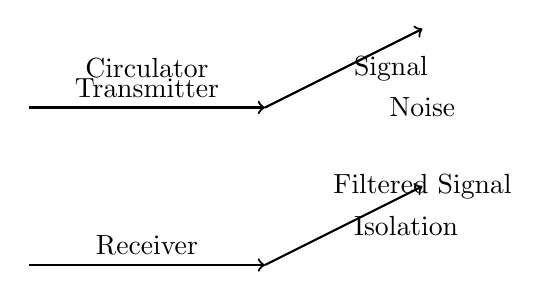
\begin{tikzpicture}
    \draw [->, thick] (0,0) -- (3,0) node[midway, above] {Transmitter};
    \draw [->, thick] (0, -2) -- (3, -2) node[midway, above] {Receiver};
    \draw [->, thick] (3, 0) -- (5, 1) node[midway, right] {Signal};
    \draw [->, thick] (3, -2) -- (5, -1) node[midway, right] {Isolation};
    
    \node at (1.5,0.5) {Circulator};
    \node at (5,0) {Noise};
    \node at (5,-1) {Filtered Signal};
\end{tikzpicture}
\end{center} 

This diagram illustrates the role of the circulator in directing signals while maintaining isolation, thereby addressing intermodulation interference effectively.